\subsection{Normals}
For each triangle $T=[p_1, p_2, p_3]$ of a triangle mesh, the normal is defined as
$$n(T) = \frac{(p_2 - p_1) \times (p_3 - p_1)}{||(p_2 - p_1) \times (p_3 - p_1)||}$$
The normal along each edge $E$ is the halfway between the normals of two adjacent triangles $T_1$ and $T_2$
$$n(E) = \frac{n(T_1) + n(T_2)}{||n(T_1) + n(T_2)||}$$
The normal at vertex $V$ is obtained averaging the normals of the $n$ adjacent triangles
$$n(V) = \frac{\sum_{i =1}^n \gamma_i n(T_i)}{||\sum_{i =1}^n \gamma_i n(T_i)||}$$
Where $\gamma_i$ can be a constant value, equal to the triangle area or equal to the angle $\theta_i$ of $T_i$ at $V$.
\cite{geometryprocessing}
%%%%%%%%%%%%%%%%%%%%%%%%%%%%%%%%%%%%%%%%%%%%%%%%%%%%%%%%%%%%%%%%%

\subsection{Local averaging regions} \label{section:localaveraging}
A mesh can be constructed either as the limit of a family of smooth surfaces or as a linear approximation of an arbitrary surface. To derive a spatial average of geometric properties we mix finite elements (a linear interpolation between three vertices of a triangle) and finite volumes (finite-volume region on a triangulated surface using Voronoi cells or Barycentric cells, Fig. \ref{fig:localregions}). Restricting the average to the neighboring triangles (\textit{1-ring}) we can choose for each vertex an associated surface patch over which the average will be computed.
Let $\mathcal{A}_{Barycenter}$ be the area formed using barycenters and $\mathcal{A}_{Voronoi}$ the one formed using \textit{Voronoi} cell. The general case is represented by a point that can be anywhere, let's denote this surface area $\mathcal{A}_M$.

\begin{figure}[!h]
    \centering
    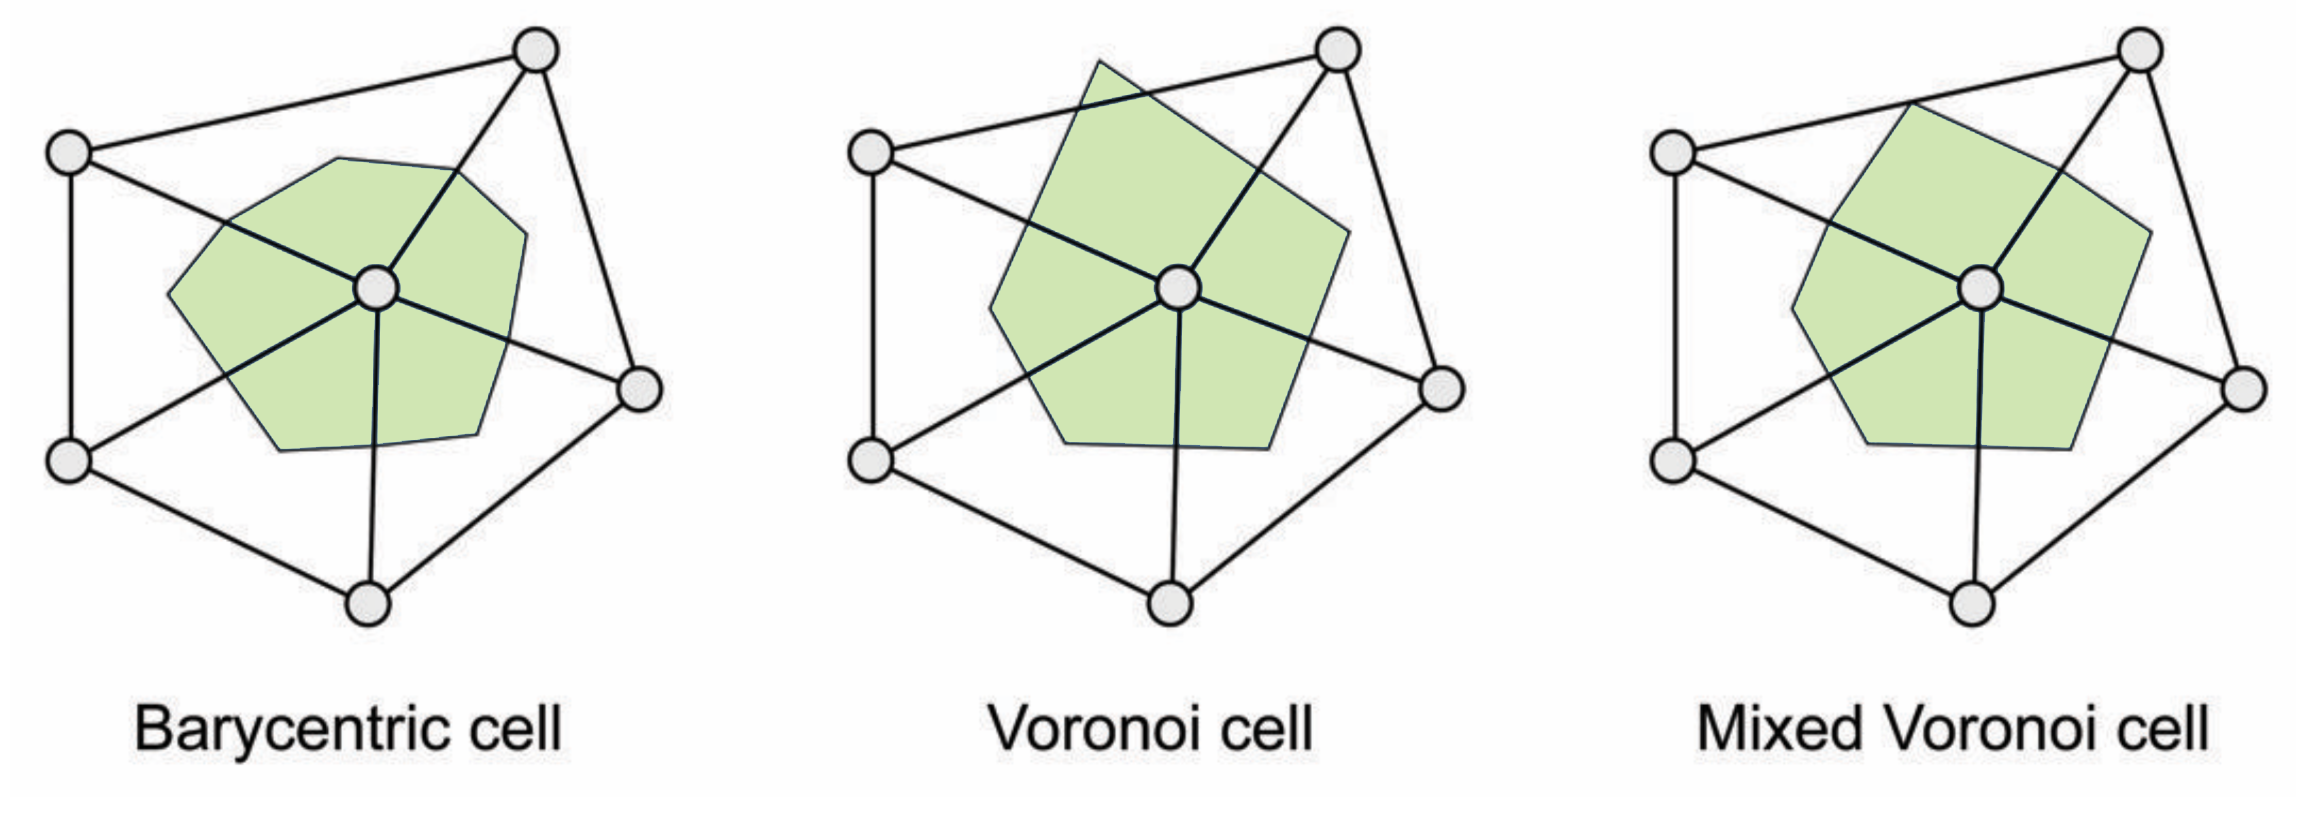
\includegraphics[scale=0.35]{images/localregions.png}
    \label{fig:localregions}
    \caption{Local averaging regions used for computing discrete differential operators associated with the center vertex of the one-ring neighborhood. \cite{polygonmeshprocessing}}
\end{figure}
\textit{Voronoi} cell of each vertex is an appropriate local region that provide a stable error bounds.
The \textit{Voronoi} region for a point $P$ of a triangle non-obtuse $[P, Q, R]$ is expressed as $\frac{1}{8}(| PR|^2 cot \angle Q + |PQ |^2 cot \angle R)$. The sum of these areas for the whole \textit{1-ring neighborhood} gives the non-obtuse \textit{Voronoi} area for a vertex. The above expression for the \textit{Voronoi} finite-volume area does not hold in case of obtuse angles. Let's define a new surface area for each vertex denoted $\mathcal{A}_{Mixed}$. Essentially the idea is to use the circumcenter point for each non-obtuse triangle and to use the midpoint of the edge opposite to the obtuse angle in case of an obtuse triangle. (See Pseudocode \ref{appendix:localaveraging}). \cite{meshlab}

\subsection{Gaussian Curvature} \label{section:gaussian-curvature-intro}
The \textit{Gaussian curvature} $K$ is defined as the product of the principal curvatures (square of the geometric mean):
$$K=k_1k_2$$
where $k_1$ and $k_2$ are the principal directions. A basic interpretation should be to imagine the \textit{Gaussian curvature} like a logical \texttt{AND} since it will check if there is a curvature along both directions.
The curvature of a surface is characterized by the principal curvatures, the \textit{Gaussian curvature} and the \textit{mean curvature} are simply averages of them.
\cite{WEBSITE:gaussiancurvaturedirty}
%---------
\begin{figure}[!h]
  \centering
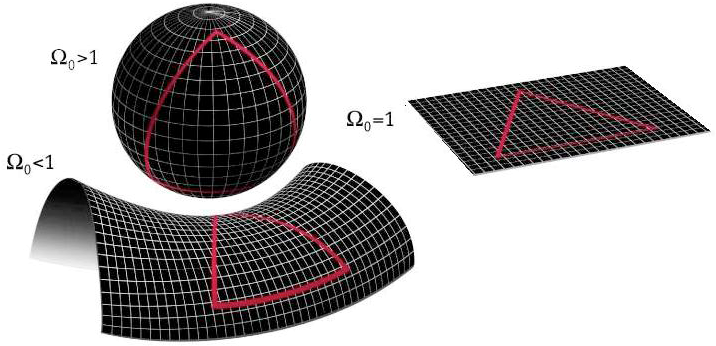
\includegraphics[scale=0.5]{images/gaussian_curvature_examples.png}
\caption{Positive curvature, negative curvature and zero curvature.}\label{fig:curvature-gaussian}
\end{figure}
Surfaces that have a zero gaussian curvature are called \textit{developable surfaces} because they can be flattened out into the plane without any stretching. \textit{Gaussian curvature} should be zero inside each mesh triangle and the same along edges since it can be flattened symmetrically into the plane by simply rotating one triangle about the common edge into the plane defined by the other. Consequently the \textit{Gaussian curvature} is concentrated at the vertices of a triangle and defined as the \textit{angle defect}
$$K(V) = 2 \pi - \sum_{i=1}^n \theta_i$$
where $\theta_i$ are the angles of the triangle $T_i$ adjacent to the vertex $V$ at $V$. This should be seen as the integral of the Gaussian curvature over a certain region $S(V)$ around $V$, where these $S(V)$ form a partition of the surface of the entire mesh.
$$ K(V) = \int_{S(V)} KdA  $$
\textit{Negative curvature} can be recognized by the fact that external directions curve in opposite directions, \textit{zero curvature} has one external direction that has zero curvature, \textit{positive curvature} has external directions that curve in the same direction (Fig. \ref{fig:curvature-gaussian}).
The \textit{Theorema Egregium}, discovered by C.F. Gauss in 1827, states that the \textit{Gaussian curvature} is an intrinsic property of the surface that does not depend on the space, despite by the fact that is define as the product of the principal curvatures (whose value depends on how the surface is immersed in the space). Technically, the \textit{Gaussian curvature} is invariant under isometries.
We can then notice that triangle angles add up to less than $180 \degree$ in negative curature, exactly $180 \degree$ in zero curature, and more than $180 \degree$ in positive curature.
\cite{geometryprocessing}
%%%%%%%%%%%%%%%%%%%%%%%%%%%%%%%%%%%%%%%%%%%%%%%%%%%%%%%%%%%%%%%%%

\subsection{Mean Curvature}
The \textit{mean curvature} H is defined as the arithmetic mean of principal curvatures : $$H = \frac{k_1 + k_2}{2}$$ where $k_1$ and $k_2$ are the principal directions. A basic interpretation should be to imagine the \textit{mean curvature} like a logical \texttt{OR} since it will check if there is a curvature along at least one direction.\cite{WEBSITE:gaussiancurvaturedirty}
The \textit{mean curvature} inside each mesh triangle is zero, but it does not vanish at edges. The \textit{mean curvature} associated with an edge is defined as $H(E) = \parallel E \parallel {\theta}_E/2$ where ${\theta}_E/2$ is the signed
angle between the normals of adjacent triangles (see Fig. \ref{fig:mean-curvature}).

\begin{figure}[h]
  \centering
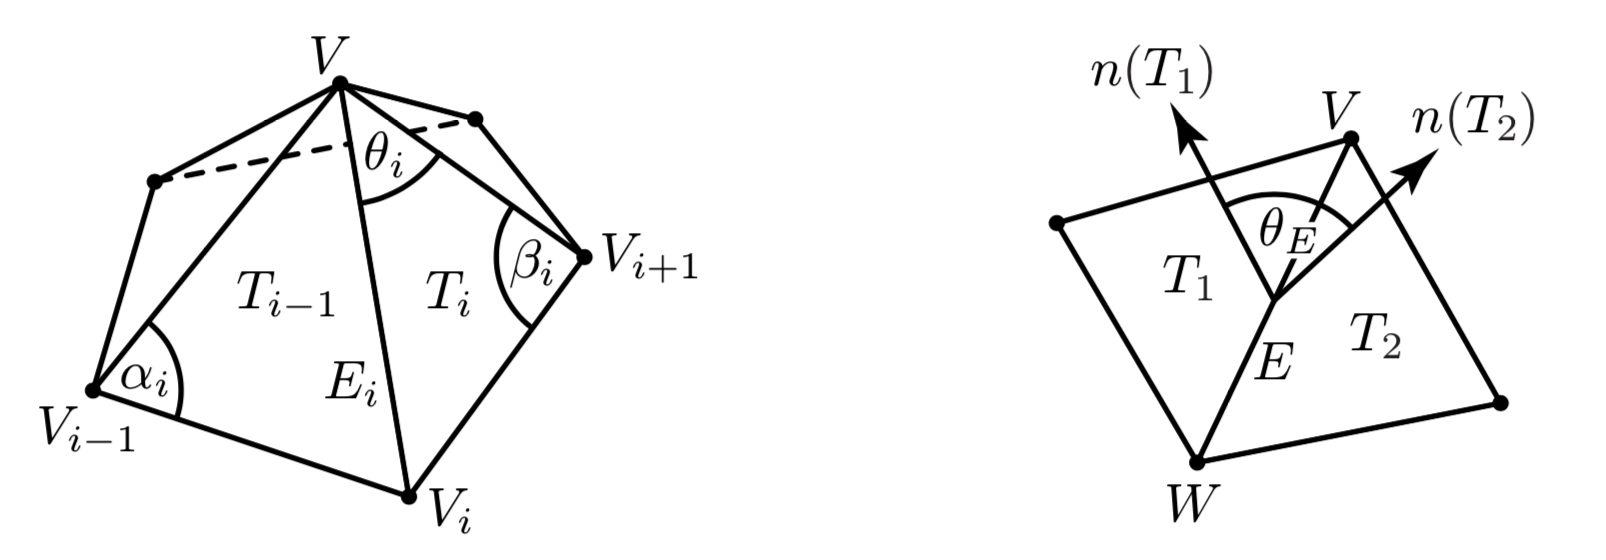
\includegraphics[scale=0.4]{images/mean_curvature_paper.png}
\caption{A vertex $V$ with its neighbouring vertices $V_i$ and adjacent triangles $T_i$. Angles opposite the edge $E_i$ are denoted by $\alpha_i$ and $\beta_i$. The
angle between the normals of adjacent triangles $T_1$ and $T_2$ with positive or negative sign is denoted as ${\theta}_E$.\cite{geometryprocessing}}\label{fig:mean-curvature}
\end{figure}
Let's think of an edge as a cylindrical patch $C(E)$ with a radius $r$ that touches the planes defined by adjacent triangles. The \textit{mean curvature} at any point of the cylindrical patch is defined as $1/(2r)$ and the area of $C(E)$ is $r||E||\theta_E$
$$H(E) = \int_{C(E)} HdA$$. The \textit{mean curvature} at a vertex $V$ is defined as $$H(V) = \frac{1}{2} \sum_{i=1}^n H(E_i)$$ Averaging the mean curvatures of its adjacent edges guarantee that \textit{mean curvature} of an edge is divide uniformly to both end points. $H(E)$ and $H(V)$ should be seen as integral curvature values associated to regions $S(E)$ and $S(V)$.
\cite{geometryprocessing}

%%%%%%%%%%%%%%%%%%%%%%%%%%%%%%%%%%%%%%%%%%%%%%%%%%%%%%%%%%%%%%%%%

\subsection{Mean Curvature Vector}
Let be $H = H n$ the surface normal vector scaled by the \textit{mean curvature} to derive the discrete mean curvature vector associated to the mesh edge $E=[V, W]$
$$ H(E) = \int_{C(E)} HdA = \frac{1}{2} (V-W) \times (n(T_1) - n(T_2))$$
The length of $H(E)$ gives the edge mean curvature $H(E) = ||H(E) || = ||E|| sin(\theta_E/2)$. The discrete mean curvature vector associated to $V$ can be obtained averaging $H(E)$ over the edges adjacent to a vertex $V$
$$H(V) = \frac{1}{2} \sum_{i=1}^{n} H(E_i) = \frac{1}{4}\sum_{i=1}^n (\cot \alpha_i + \cot \beta_i)(V - V_i)$$
where $\alpha_i$ and $\beta_i$ are angles opposite to $E_i$ (see Fig. \ref{fig:mean-curvature}).
\cite{geometryprocessing}
